\documentclass[11pt,a4paper]{article}
\usepackage{fullpage}
\usepackage{graphicx}
\usepackage{float}
\usepackage{enumitem}
\usepackage{caption}
\usepackage{amsmath}
\newcommand*{\addheight}[2][.5ex]{%
  \raisebox{0pt}[\dimexpr\height+(#1)\relax]{#2}%
}
\usepackage{datetime}
\newdate{date}{02}{02}{2016}
\date{\displaydate{date}}
\title{\textbf{Chaotic Dynamics - CSCI 5446} \\
Problem Set 3}
\author{Santhanakrishnan Ramani}
\begin{document}
\maketitle

\section*{Problem 0}
\begin{figure}[H]
{
The Figure \ref{fig:prob0} represents the an interesting part of "Newton's method on $x^3 - 1 = 0$" plot from the Julia site. \par\bigskip
\centering 
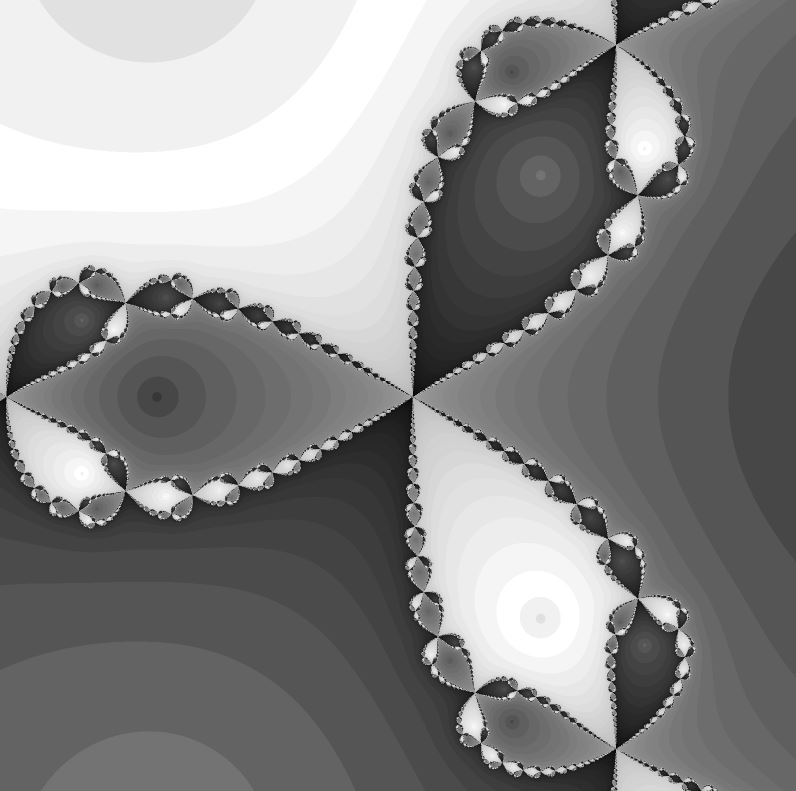
\includegraphics[scale=0.8]{images/julia.jpg}
\caption{Julia plot}\par\medskip
\label{fig:prob0}
}
\end{figure}

\section*{Problem 1}
\paragraph*{•}
Capacity Dimension of the middle sixth removed Cantor Set.
\begin{center}
\begin{tabular}{ |c|c|c| } 
 \hline 
 K & $N(\epsilon)$ & $\epsilon$ \\
 \hline 
 0 & 1 & 1 \\ 
 1 & 5 & 1/6 \\
 2 & 25 & 1/36 \\
 . & . & . \\
 $K$ & $5^K$ & $(1/6)^K$\\
 \hline
\end{tabular}
\end{center}
\begin{align*}
d_c = & \lim_{\epsilon \to 0} \frac{\log(N(\epsilon))}{\log(\frac{1}{\epsilon})}\\
d_c = &\lim_{k \to \infty} \frac{\log(5^{k})}{\log(6^{k})}\\
d_c = &\frac{\log(5)}{\log(6)} = 0.898
\end{align*}

\section*{Problem 2}
\begin{enumerate}[label=(\alph*)]

\item 
Transform the following third order ODE into three first-order ODEs \\
$$2x''' - 3{\tan(\frac{x''}{2})} + 16{\log(x')} - x = 0$$
Let the helper variables be, 
$$x' = y$$
$$y' = z$$
First Order ODE's
\begin{align*}
x' &= y\\
y' &= z\\
z' &= \frac{1}{2}[3{\tan(\frac{z}{2})} - 16{\log(y)} + x]
\end{align*}

\item 
Transform the following set of first-order ODEs into a single higher-order ODE,
\begin{align*}
x' &= y\\
y' &= z\\
z' &= yz + \log(y)\\
\end{align*}
Higher Order ODE is
$$ x''' - {x'}{x''} -\log(x') = 0$$

\item
Both the Systems in (a) and (b) are nonlinear.
\par\medskip
\textbf{Reason}\par\medskip
When the System was expressed in terms of first order ODEs,\\(a) has \textit{log} term in state variable $z'$,\\(b) has product term $yz$ in state variable $z'$\\ which makes the whole system non linear.

\end{enumerate}
\newpage
\section*{Problem 3}

\begin{enumerate}[label=(\alph*)]

\item 
The Figure \ref{fig:prob3a} represents the self-similar "Fractal Tree" that was obtained by running the code for 13 iterations. \par\bigskip
\begin{minipage}{\linewidth}
{
\centering 
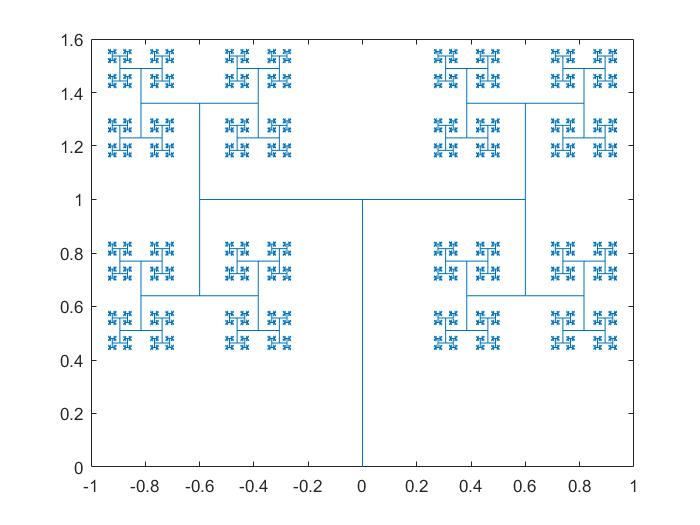
\includegraphics[scale=0.4]{images/prob3a.jpg}
\captionof{figure}{Fractal Tree}
\label{fig:prob3a}
}
\end{minipage}
\par\medskip
Capacity dimension of the fractal composed of the leaves of this tree.
\begin{center}
\begin{tabular}{ |c|c|c| } 
 \hline 
 K & $N(\epsilon)$ & $\epsilon$ \\
 \hline 
 0 & 1 & 1 \\ 
 1 & 2 & 3/5 \\
 2 & 4 & 9/25 \\
 . & . & . \\
 $K$ & $2^K$ & $(3/5)^K$\\
 \hline
\end{tabular}
\end{center}
$$d_c = \lim_{\epsilon \to 0} \frac{\log(N(\epsilon))}{\log(\frac{1}{\epsilon})}$$
\centerline
{
$d_c = \lim_{k \to \infty} \frac{\log(2^{k})}{\log((5/3)^{k})}$
$d_c = \frac{\log(2)}{\log(5/3)} = 1.357$
}
\item
When the length of line segment is half as the previous line segment, then the tree looks to be thin having lesser number of branches. (Ratio = 0.5)
$$d_c = \frac{\log(2^k)}{\log(2^k)} = 1$$
When the ratio is greater than $\sqrt{2}$, the tree looks like a grid increasing in size and gap for each iteration and volume of the tree is huge. (Ratio = 1.5)

\centerline
{\textbf{Dimension can't be found as $\epsilon \to \infty$ rather than $\epsilon \to 0$}}\par\medskip
When the ratio is less than 0.5, the tree is very sparse with lesser number of branches and leaves and very small volume. (Ratio = 0.40)
$$d_c = \frac{\log(2^k)}{\log((5/2)^k)} = 0.756$$

\item
The Figure \ref{fig:prob3c} represents the self-similar "Fractal Tree" that was obtained by running the code for 10 iterations with 60 and 40 degrees for the angles and 0.7 and 0.65 for the lengths of respective sides. \\
\begin{minipage}{\linewidth}
{
\centering 
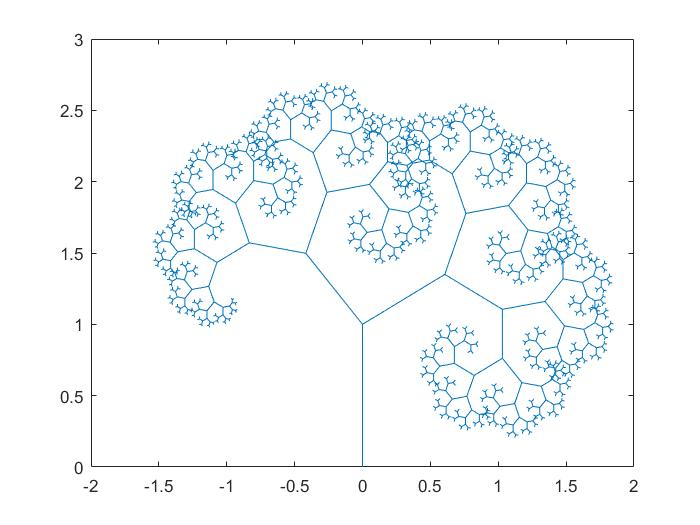
\includegraphics[scale=0.40]{images/prob3c.jpg}
\captionof{figure}{Fractal Tree}
\label{fig:prob3c}
}
\end{minipage}

\item
Some interesting plots for different angles and length.\\
\begin{minipage}{\linewidth}
{
\begin{table}[H]
\centering
\begin{tabular}{|c|c|}
	\hline
	\addheight{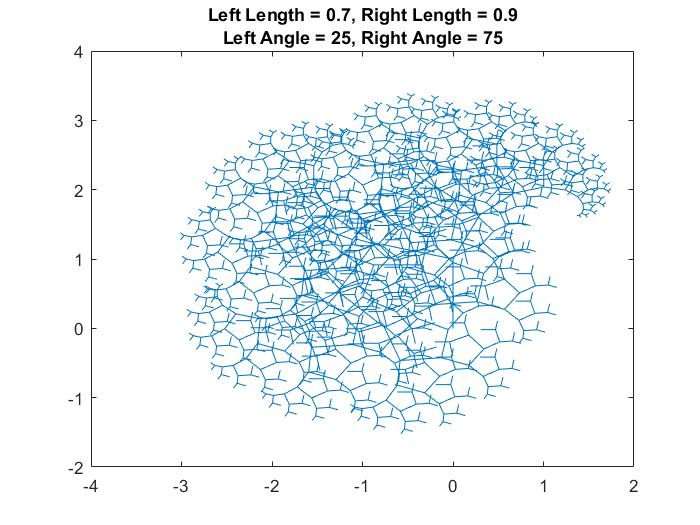
\includegraphics[width=75mm]{images/prob3d1.jpg}} &
    \addheight{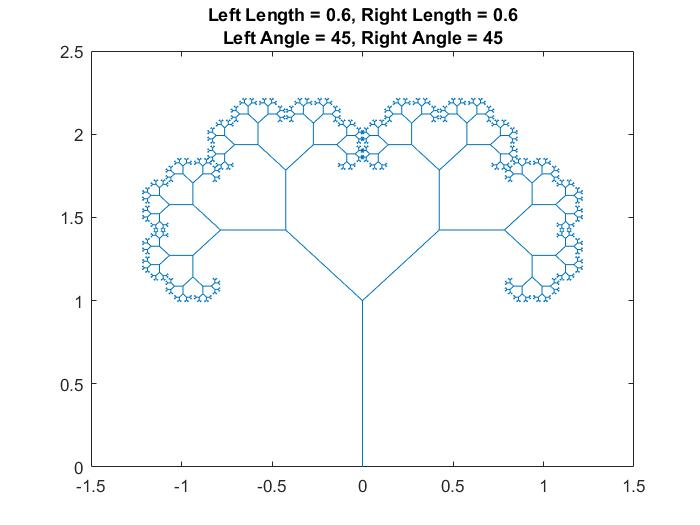
\includegraphics[width=75mm]{images/prob3d2.jpg}} \\
    \hline
    \addheight{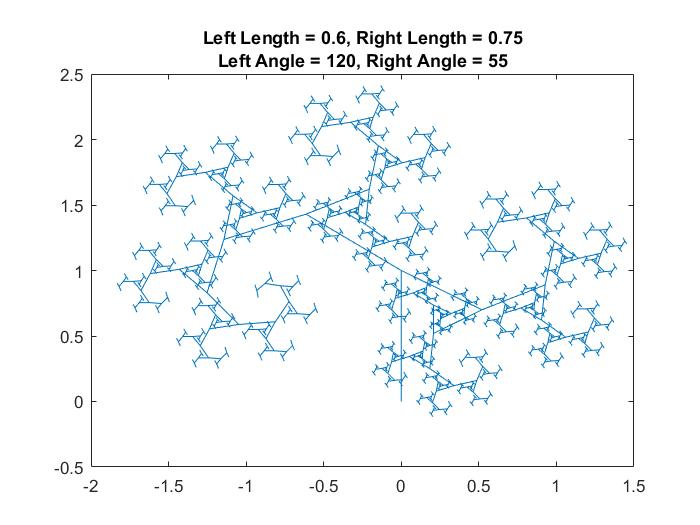
\includegraphics[width=75mm]{images/prob3d3.jpg}} &
    \addheight{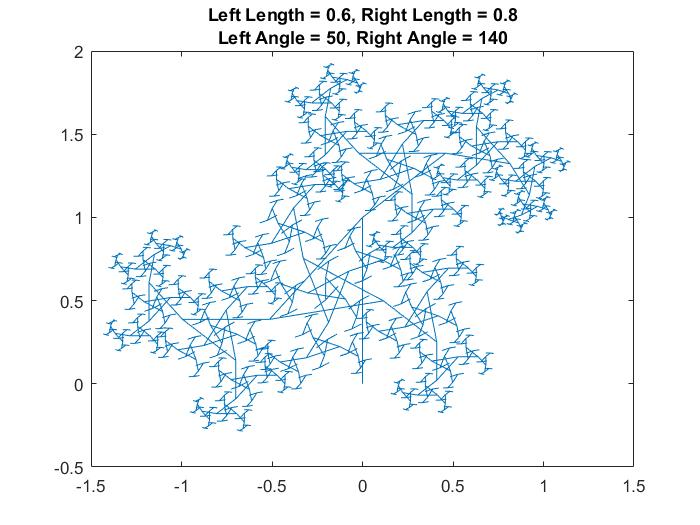
\includegraphics[width=75mm]{images/prob3d4.jpg}} \\
	\hline
\end{tabular}
\end{table}
}
\end{minipage}
\end{enumerate}
\end{document}
